\chapter{Stimmabgabe}
Die Stimmabgabe im Wahlinformationssystem l�uft folgenderma�en ab. Der W�hler erscheint im Wahllokal seines Wahlbezirkes. 
Dort legt er seinen Personalausweis vor. Durch die Vorlage des Personalausweises wird verhindert dass eine nicht-autorisierte
Person eine Stimme abgeben kann. Der Wahlhelfer vor Ort gibt die Personalausweisnummer in der vorgesehenen Weboberfl�che ein: 

\begin{figure}[htbp]
\centering
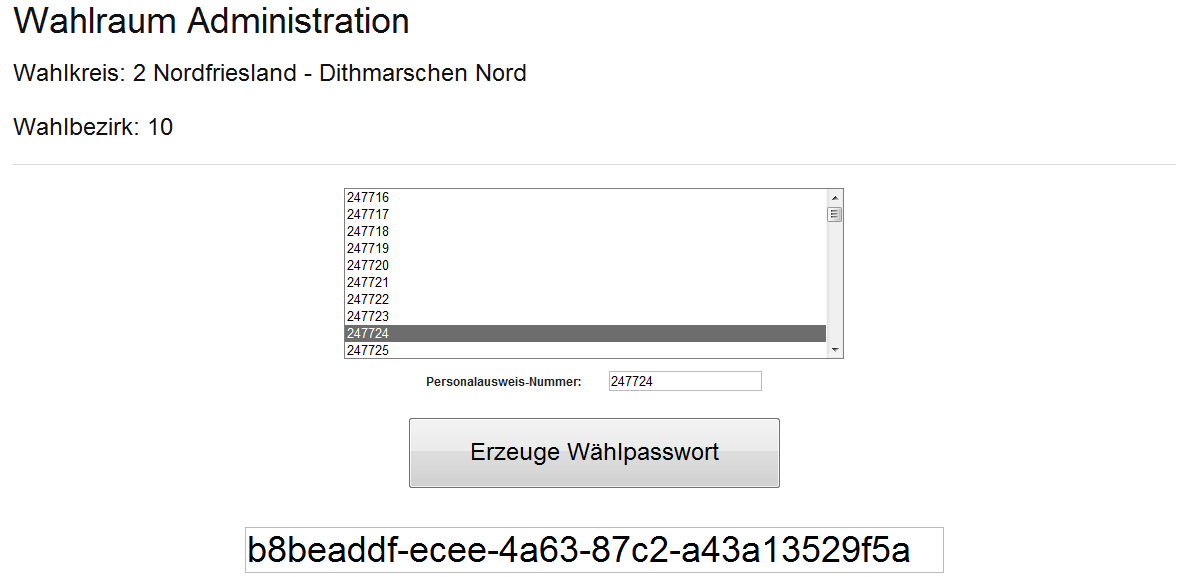
\includegraphics[width=0.4\textwidth]{figures/wahlraum-screenshot.png}
\caption{Webschnittstelle zur Eingabe der Personalausweis-Nummer}
\label{fig:wahlraum-screenshot}
\end{figure}

Das System pr�ft ob die Personalausweisnummer ein stimmberechtigter W�hler ist (Ausweisnummer vorhanden). Wenn ja, wird gepr�ft ob dieser nicht 
bereits seine Stimme abgegeben hat (Flag \emph{gew�hlt} muss auf \emph{false} gesetzt sein). Hat er noch nicht gew�hlt, generiert das System ein 
zuf�lliges, zentral auf dem Server gespeichertes W�hlpasswort, das der Wahlhelfer dem W�hler auf einem Zettel �bergibt. 
Durch die Generierung des W�hlpassworts wird das Flag \emph{gew�hlt} auf \emph{true} gesetzt. Dadurch wird verhindert dass der gleiche 
W�hler mehrfach w�hlen kann. 

\newpage

Das W�hlpasswort berechtigt den W�hler an einem Wahlcomputer seine Stimme abzugeben:

\begin{figure}[htbp]
\centering
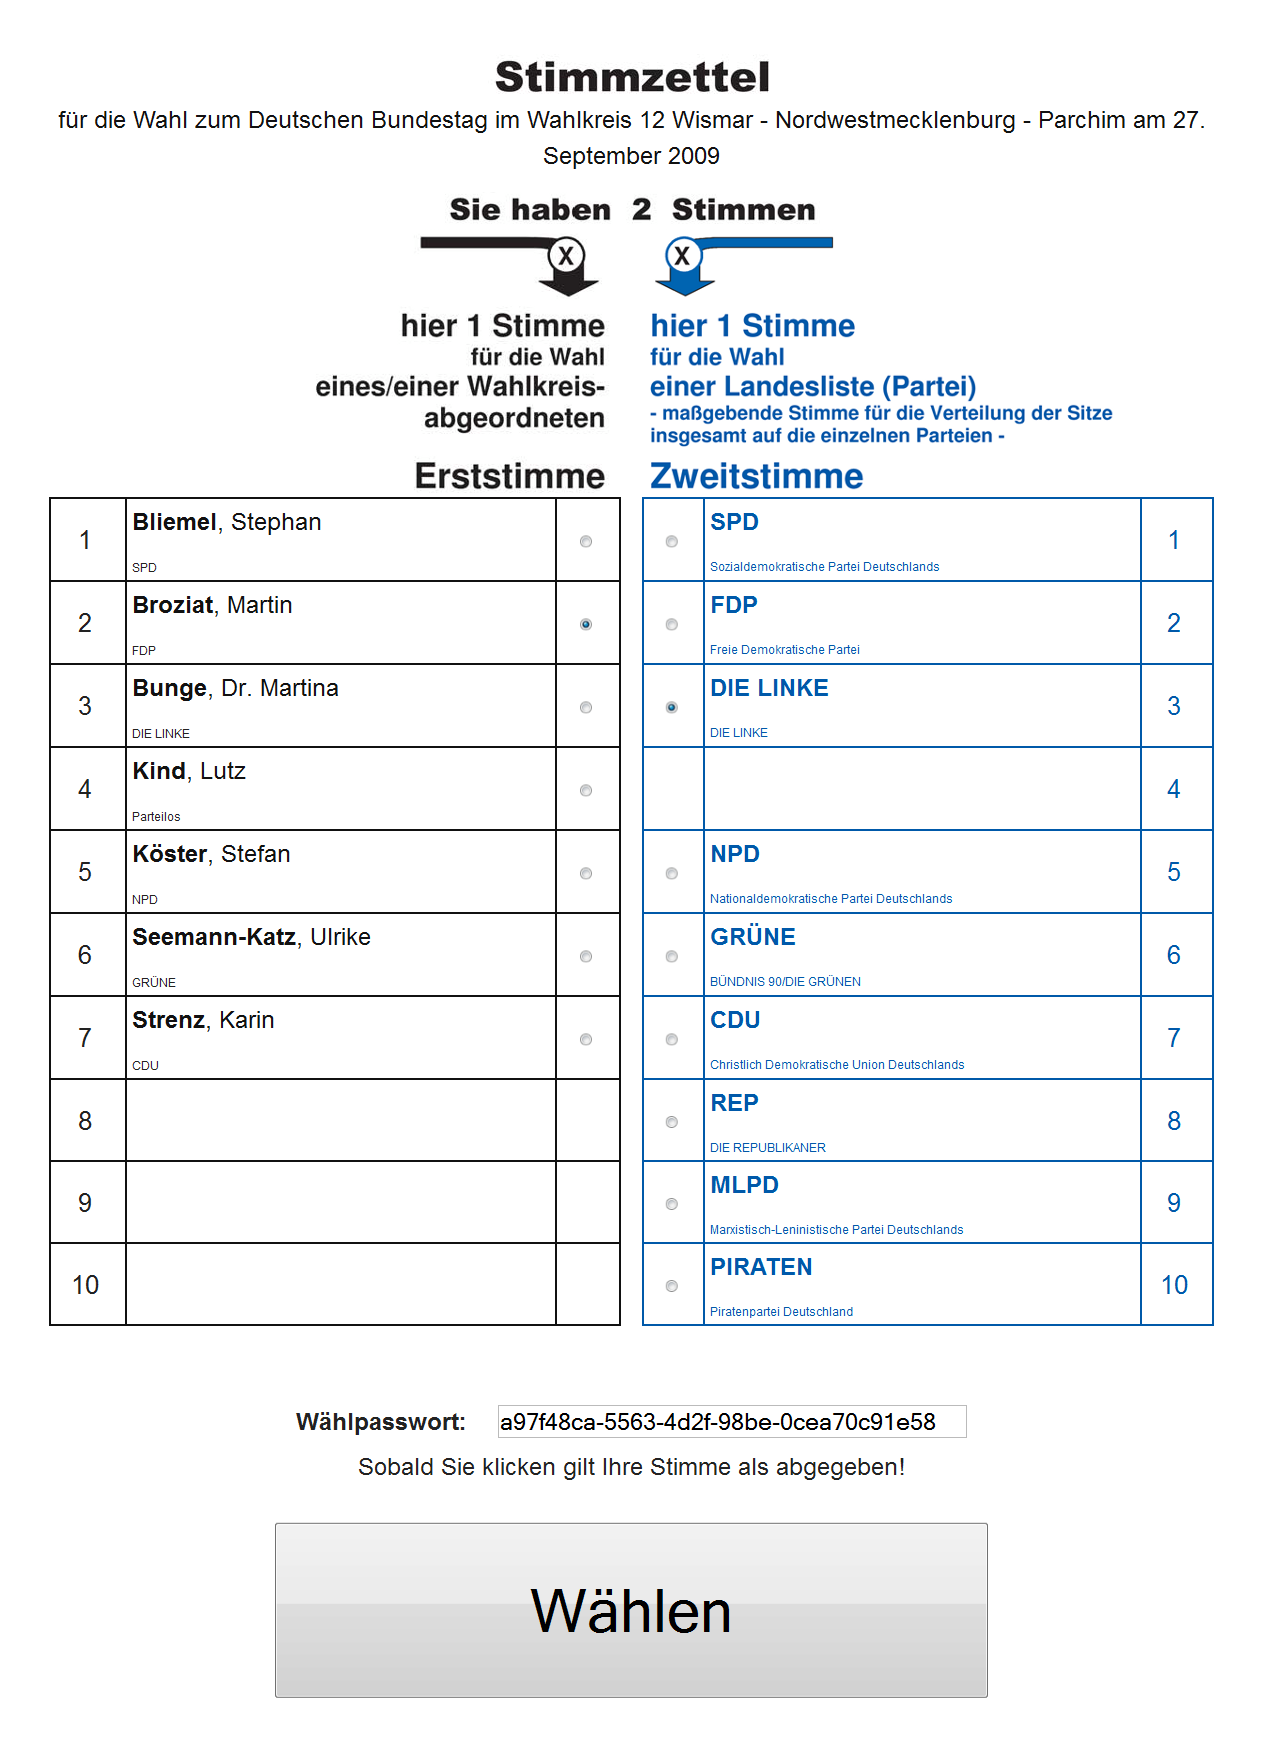
\includegraphics[width=0.85\textwidth]{figures/wahlzettel-screenshot.png}
\caption{Digitaler Wahlzettel mit W�hlpasswort}
\label{fig:wahlzettel-screenshot}
\end{figure}

Sobald der W�hler seine Kreuze gemacht hat, �berpr�ft das
System das eingegebene W�hlpasswort. Wenn es korrekt ist, wird die Stimme gez�hlt und das W�hlpasswort erlischt. Durch die Indirektion �ber das anonyme W�hlpasswort wird
maximaler Datenschutz gew�hrleistet. 

Alle �bertragungen vom Wahllokal zum Server m�ssen gesichert sein. Da sichere Verbindungen nicht Thema dieses Projektes sind, 
wird in der Implementierung davon ausgangen, dass die Sicherung der Verbindung au�erhalb erfolgt.